\Subsection{Билет 101: Произведение полуколец. Параллелепипеды и ячейки. Связь между ними.}

\begin{definition}\thmslashn
	
	Декартово произведение полуколец.
	
	$\mathcal{P}, \mathcal{Q}$ -- полукольца подмножеств $X$ и $Y$ соответственно.
	
	
	$\mathcal{P} \times \mathcal{Q} = \{P\times Q \;\;:\;\; P \in \mathcal{P}, \; Q\in\mathcal{Q} \}$ -- семейство подмножеств $X\times Y$.
\end{definition}

\begin{theorem}\thmslashn
	
	Декартово произведение полуколец -- полукольцо.
\end{theorem}

\begin{proof}\thmslashn
	
	(скорее махание руками, чем доказательство)
	
    Нужно проверить свойства полукольца.

    \begin{enumerate}
        \item 
	$\emptyset = \emptyset \times \emptyset \in \mathcal{P} \times \mathcal{Q}$
	    \item 
	$(P\times Q) \cap (\tilde{P} \times\tilde{Q}) = (P \cap \tilde{P}) \times (Q\cap \tilde{Q})$

    Пересечение декартовых произведение - декартово произведение пересечений. Можно посмотреть на картинки ниже и понять. 

    +- формально: $(a, b) \in (P \times Q) \iff a \in P, b \in Q$, аналогично $(a,b) \in (\tilde{P} \times \tilde{Q}) \iff a \in \tilde{P}, b \in \tilde{Q}$.

    Тогда $a \in (P \times Q) \cap (\tilde{P} \times \tilde{Q}) \iff$ ($a \in P$ и $a \in \tilde{P}$), и ($b \in Q$ и $b \in \tilde{Q}$) $\iff (a, b) \in (P \cap \tilde{P}) \times (Q \cap \tilde{Q})$
	
	    \item
	Рисуем картинки. Это два прямоугольника, один вычитаем из другого. Нужно понять, что разность представляется в виде объединения прямоугольников.
	
	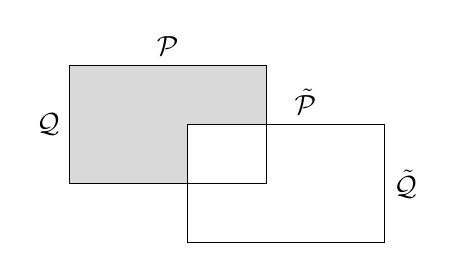
\begin{tikzpicture}[scale=0.5]
	\begin{scope}
	\clip (0, 0) rectangle (5, 3);
	\fill[gray!30] (0, 0) rectangle (5,3);
	\fill[white] (3, 1.5) rectangle (8, -1.5);
	\end{scope}
	\draw (0, 0) rectangle (5, 3);
	\draw (3, 1.5) rectangle (8, -1.5);
	\node[above] at (2.5, 3) {$\mathcal{P}$};
	\node[left] at (0, 1.5) {$\mathcal{Q}$};
	\node[above] at (6, 1.5) {$\tilde{\mathcal{P}}$};
	\node[right] at (8, 0) {$\tilde{\mathcal{Q}}$};
	\end{tikzpicture}
	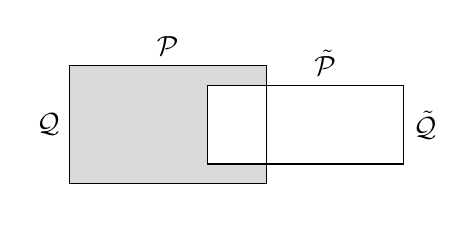
\begin{tikzpicture}[scale=0.5]
	\begin{scope}
	\clip (0, 0) rectangle (5, 3);
	\fill[gray!30] (0, 0) rectangle (5,3);
	\fill[white] (3.5, 2.5) rectangle (8.5, 0.5);
	\end{scope}
	\draw (0, 0) rectangle (5, 3);
	\draw (3.5, 2.5) rectangle (8.5, 0.5);
	\node[above] at (2.5, 3) {$\mathcal{P}$};
	\node[left] at (0, 1.5) {$\mathcal{Q}$};
	\node[above] at (6.5, 2.5) {$\tilde{\mathcal{P}}$};
	\node[right] at (8.5, 1.5) {$\tilde{\mathcal{Q}}$};
	\node at (0, -0.5) {};
	\end{tikzpicture}
	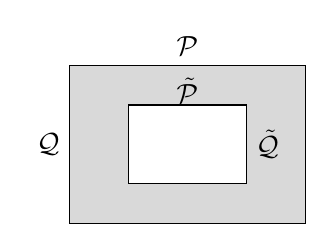
\begin{tikzpicture}[scale=0.5]
	\begin{scope}
	\clip (0, 0) rectangle (6, 4);
	\fill[gray!30] (0, 0) rectangle (6, 4);
	\fill[white] (1.5, 1) rectangle (4.5, 3);
	\end{scope}
	\draw (0, 0) rectangle (6, 4);
	\draw (1.5, 1) rectangle (4.5, 3);
	\node[above] at (3, 4) {$\mathcal{P}$};
	\node[left] at (0, 2) {$\mathcal{Q}$};
	\node[above] at (3, 2.8) {$\tilde{\mathcal{P}}$};
	\node[right] at (4.5, 2) {$\tilde{\mathcal{Q}}$};
	\end{tikzpicture}
	
	Порисовав картинки, понимаем, что:
	
	$(P\times Q) \setminus (\tilde{P} \times\tilde{Q}) = P\times (Q\setminus \tilde{Q}) \sqcup (P\setminus \tilde{P}) \times (Q\cap \tilde{Q})$
	
	А это лежит в $\mathcal{P} \times \mathcal{Q}$: оба дизъюнкткных множества выше можно разбить на дизъюнктные объединения, ведь каждое из них является декартовым произведением множеств из полукольца или дополнением. Дополнения разбиваются по 3 свойству полукольца.

    \begin{remark}
        На нашей лекции Храбров неправильно выписал формулу выше.
    \end{remark}
    \end{enumerate}
\end{proof}


\begin{definition}\thmslashn
	
	$\R^n$
	
	Замкнутый параллелепипед -- $[a_1,b_1]\times[a_2, b_2]\times...\times[a_n, b_n] =: [a,b]$
	
	$a = [a_1,a_2,...,a_n]$
	
	$b = [b_1, b_2,...,b_n]$
	
	
	Открытый параллелепипед -- $(a_1,b_1)\times(a_2, b_2)\times...\times(a_n, b_n) =: (a,b)$
	
	
	Ячейка -- $[a_1,b_1)\times[a_2, b_2)\times...\times[a_n, b_n) =: [a,b)$
	
	Обозначения. 
	
	$\mathcal{P}^n$ -- множество всех ячеек из $\R^n$
	
	$\mathcal{P}^n_{\Q}$ -- множество всех ячеек из $\R^n$ с рациональными координатами вершин.
\end{definition}

\begin{theorem}\thmslashn
	
	Непустая ячейка представима в виде пересечения счетного множества открытых параллелепипедов и представима в виде счетного объединения замкнутых.
\end{theorem}

\begin{proof}\thmslashn
	
	$[a,b) = [a_1,b_1) \times...\times [a_n, b_n)$
	
	$C_k := (a_1 - \frac1k, b_1) \times ...\times (a_n-\frac1k, b_n)$
	
	$\bigcap\limits_{k=1}^{\infty} C_k = [a,b)$:

    $\bigcap\limits_{k=1}^{\infty} C_k \supset [a,b)$, так как $C_k \supset [a,b) \forall k$
    
    $\bigcap\limits_{k=1}^{\infty} C_k \subset [a,b)$, так как если $\exists x \in C_k, x \notin [a,b)$, то начиная с некоторого номера $x \notin \bigcap\limits_{k=1}^{n} C_k$, так как они сужаются

	$D_k := [a_1, b_1 - \frac1k]\times...\times [a_n, b_n - \frac1k]$
	
	$\bigcup\limits_{k=1}^{\infty}D_k = [a,b)$

    Доказательство аналогично: $\subset$ очевиден, а $\supset$ т.к. начиная с некоторого номера каждая точка попадёт в объединение
\end{proof}
